\documentclass[11pt]{beamer}
\usetheme{Pittsburgh}
\usepackage{xcolor}
\usepackage{pifont,enumitem}
\usepackage{etoolbox}
\usepackage{textpos}
\usepackage{capt-of}% or use the larger `caption` package
%\usepackage[pass]{geometry} 
\usepackage{multirow}
\usepackage{hhline} 
\usepackage{colortbl}
\usepackage{tikz}
\usetikzlibrary{trees,automata,positioning}
\usepackage{verbatim}
\usepackage{mathdots}

\setbeamertemplate{frametitle}{%
    \nointerlineskip%
    \usebeamerfont{frametitle}%
    \begin{beamercolorbox}[wd=\paperwidth,ht=1cm,sep=3pt]{frametitle}

        \includegraphics[height=1.2\baselineskip]{"VOUW logo-03"}
        \hfill\usebeamerfont{frametitle}\insertframetitle%

    \end{beamercolorbox}
}

\setbeamercolor{frametitle}{fg=red!45!yellow,bg=teal!75}
\setbeamercolor*{title}{fg=teal!75}
\usepackage{microtype}
\usepackage[utf8]{inputenc}

% import from STIX
\DeclareFontEncoding{LS1}{}{}
\DeclareFontSubstitution{LS1}{stix}{m}{n}
\DeclareFontFamily{LS1}{stixfrak}{\skewchar\font127 }
\DeclareFontShape{LS1}{stixfrak}{m}{n} {<-> stix-mathfrak}{}
\newcommand{\tplus}{\text{\usefont{LS1}{stixfrak}{m}{n}\symbol{"EB}}}
\newcommand{\tminus}{\text{\usefont{LS1}{stixfrak}{m}{n}\symbol{"EC}}}
%%%

\usepackage{amsmath}
\usepackage{amsfonts}
\usepackage{amssymb}
\usepackage{graphicx}
\usepackage[T1]{fontenc}
\usepackage{lmodern}
\usepackage{MnSymbol}

\setlist[itemize]{label={\color{red!45!yellow}\Pifont{pzd}{\char93}}}
\renewcommand{\mark}[1]{\textcolor{red!45!yellow}{\textbf{#1}}}
\renewcommand{\bold}[1]{\textcolor{teal}{\textbf{#1}}}

% Set the overall layout of the tree
\tikzstyle{level 1}=[level distance=3.0cm, sibling distance=1.3cm]
\tikzstyle{level 2}=[level distance=3.5cm, sibling distance=1.3cm]
\tikzstyle{level 3}=[level distance=3.5cm, sibling distance=1.3cm]

% Define styles for bags and leafs
\tikzstyle{l1} = [rectangle, text width=3em, text centered]
\tikzstyle{l2} = [rectangle, text width=5em, text centered]
\tikzstyle{l3} = [rectangle, text width=5em, text centered]

\author{Micky Faas}
\title{Pattern Mining on Matrices}
%\setbeamercovered{transparent} 
%\setbeamertemplate{navigation symbols}{} 
%\logo{} 
%\institute{} 
%\date{} 
%\subject{} 

\begin{document}
\beamertemplatenavigationsymbolsempty
\begin{frame}
\nointerlineskip%
\begin{columns}
\column{\dimexpr\paperwidth}
\centering % Center table


\includegraphics[width=0.4\paperwidth]{"VOUW logo-02"} 
\maketitle
\end{columns}
\end{frame}

%\begin{frame}
%\tableofcontents
%\end{frame}
%%%%%%%%%%

\begin{frame}{Overview}
In this presentation I will:
\begin{itemize}
\item Introduce VOUW
\item Give a brief description of the formal problem
\item Explain the search method through some practical examples
\item Tell you about my goals for the future
\end{itemize}
\end{frame}

%%%%%%%%%%

% Full image slide
\begin{frame}{Introduction}
\nointerlineskip%
\begin{columns}
\column{\dimexpr\paperwidth}
\centering
\includegraphics[width=\paperwidth]{"rf-automaton"} 
\end{columns}
\medskip
Originally: similarity in Cellular Automata
\end{frame}

%%%%%%%%%%

\begin{frame}{Introduction}
Theoretical problem: given some $M\times N$ matrix $A$, we want to discover and extract recurring structure. As a means of
\begin{itemize}
\item `explaining' the data
\item similarity measure or clustering 
\end{itemize}
When compared to other pattern mining problems, we are specifically looking for
\begin{itemize}
\item Spatial relation/structure
\end{itemize}
\end{frame}

%%%%%%%%%%

\begin{frame}{Introduction}
Practical implementation: \texttt{libvouw} (library) and QVouw (GUI).\\[3em]

\centering
\includegraphics[width=.5\paperwidth]{"qvouw"} 

\end{frame}

%%%%%%%%%%

\begin{frame}{Is this just noise?}
\nointerlineskip%
%Given this `matrix', can you find any structure? 
\begin{columns}
\column{\dimexpr\paperwidth}
\centering
\includegraphics[width=.8\paperheight]{"eda1024"} 
\end{columns}
\end{frame}

%%%%%%%%%%

\begin{frame}{Patterns and Instances}

\begin{tabular}{l l p{5cm}}
Term? & Form & Encodes... \\
\hline 
\textbf{Pattern} & Submatrix of $A$ & ...relative positions of elements \\
\textbf{Offset} & $(i,j)\in M\times N$ & ...position of entire pattern\\
\textbf{Instance} & $M\times N$ matrix & ...absolute positions of elements \\
\textbf{Instantiation} & $M\times N$ matrix & ...what pattern's instance should be at which index
\end{tabular}

%%%%%%%%%%%

\begin{align*}
\underbrace{
\begin{bmatrix}
1 & \cdot \\[-.2em]
\cdot & 1
\end{bmatrix}}_{\textsf{Pattern}},
\underbrace{
\begin{bmatrix}
\cdot & \cdot & \cdot & \cdot & \cdot & \cdot  \\[-.2em]
\cdot & \cdot & \cdot & \cdot & \cdot & \cdot  \\[-.2em]
\cdot & \cdot & 1 & \cdot & \cdot & \cdot  \\[-.2em]
\cdot & \cdot & \cdot & 1 & \cdot & \cdot  \\[-.2em]
\cdot & \cdot & \cdot & \cdot & \cdot & \cdot  \\[-.2em]
\cdot & \cdot & \cdot & \cdot & \cdot & \cdot  \\
\end{bmatrix}}_{\textsf{Instance with offset }(2,2)}
\end{align*}
\end{frame}

%%%%%%%%%%

\begin{frame}{Example}
\begin{align*}
A =
\overbrace{
\begin{bmatrix}
1 & \cdot & \cdot & \cdot & \cdot & 1  \\[-.2em]
\cdot & 1 & \cdot & \cdot & \cdot & \cdot \\[-.2em]
1 & \cdot & \cdot & \cdot & 1 & \cdot  \\[-.2em]
\cdot & 1 & \cdot & \cdot & \cdot & 1  \\[-.2em]
1 & \cdot & 1 & \cdot & \cdot & \cdot  \\[-.2em]
\cdot & 1 & \cdot & 1 & \cdot & \cdot  \\
\end{bmatrix}}^{\textsf{Original matrix}},
G = 
\overbrace{
\begin{bmatrix}
X & \cdot & \cdot & \cdot & \cdot & Y  \\[-.2em]
\cdot & \cdot & \cdot & \cdot & \cdot & \cdot  \\[-.2em]
X & \cdot & \cdot & \cdot & X & \cdot  \\[-.2em]
\cdot & \cdot & \cdot & \cdot & \cdot & \cdot  \\[-.2em]
X & \cdot & X & \cdot & \cdot & \cdot  \\[-.2em]
\cdot & \cdot & \cdot & \cdot & \cdot & \cdot  \\
\end{bmatrix}}^{\textsf{Instantiation}}\\
\overbrace{
H = \{
X =
\underbrace{
\begin{bmatrix}
1 & \cdot \\[-.2em]
\cdot & 1
\end{bmatrix}}_{\textsf{Pattern}},
Y =
\underbrace{
\begin{bmatrix}
1
\end{bmatrix}}_{\textsf{Pattern}}
\}}^{\textsf{Model}}
\end{align*}
\end{frame}

%%%%%%%%%%

\begin{frame}{Building Patterns}
We can construct complex patterns by repeatedly combining simpler ones. We use instances for this as they encode the position of one pattern relative to another.

\begin{align*}
\underbrace{
\begin{matrix}
X = \begin{bmatrix}
0
\end{bmatrix} \\[1.0em]
Y = \begin{bmatrix}
1
\end{bmatrix}
\end{matrix}}_{\textsf{Singleton patterns}}
\longrightarrow
\underbrace{\begin{matrix}
\bar{X} = \begin{bmatrix}
\cdot  & \cdot & \cdot \\
0 & \cdot & \cdot \\
\cdot & \cdot & \cdot \\
\end{bmatrix} \\[1.0em]
\bar{Y} = \begin{bmatrix}
\cdot  & \cdot & \cdot \\
\cdot  & \cdot & \cdot \\
\cdot & 1 & \cdot
\end{bmatrix}
\end{matrix}}_{\textsf{Instances}}
\longrightarrow
\bar{X}+\bar{Y} =
\underbrace{
\begin{bmatrix}
\cdot  & \cdot & \cdot \\
0  & \cdot & \cdot \\
\cdot & 1 & \cdot
\end{bmatrix}}_{\textsf{Matrix sum}}
\longrightarrow
\underbrace{
\begin{bmatrix}
0  & \cdot \\
\cdot & 1 
\end{bmatrix}}_{\textsf{New pattern}}
\end{align*}
\end{frame}

%%%%%%%%%%%

\begin{frame}{Model Space}
Idea: we inductively define the model space by starting with singletons for each element of $A$. Then we repeatedly merge instances until we finally obtain a pattern that equals $A$.
\begin{itemize}
\item At the beginning we have the completely underfit model
\item We end up with a completely overfit model
\end{itemize}
\bigskip
Everything in between is a possible solution, but \emph{we want the solution that describes $A$ best.}\\[1em]
For example $A=\begin{bmatrix}0 & 1 \\ 1 & 0\end{bmatrix}$: what is the space of possible solutions?
\end{frame}

%%%%%%%%%%%

\begin{frame}{2x2 Model Space Lattice}

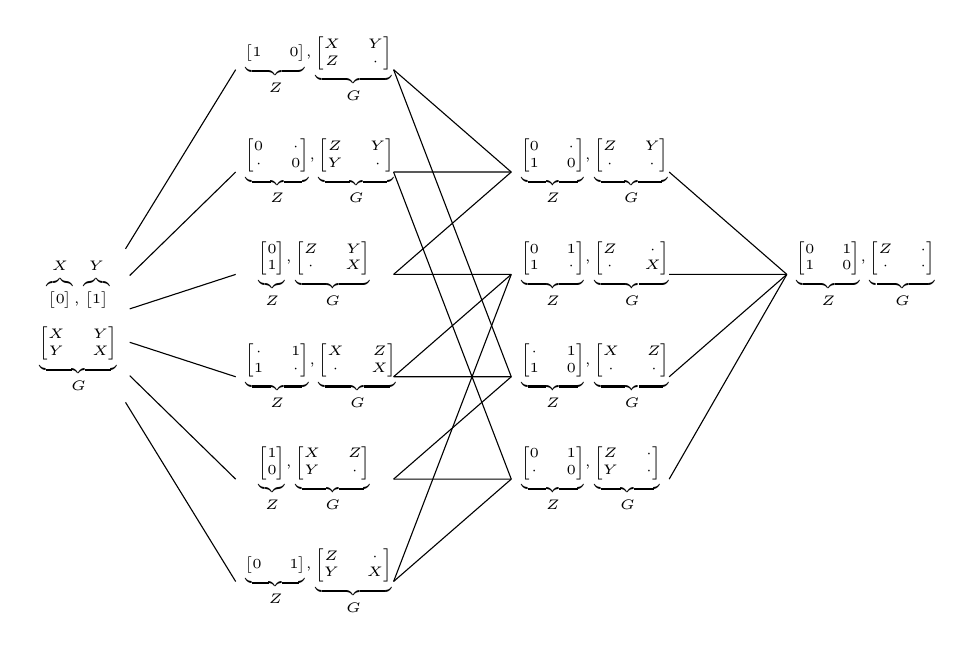
\begin{tikzpicture}[on grid, grow=right]
\node(R)[l1] {\tiny $\begin{matrix}\overbrace{\begin{bmatrix}0\end{bmatrix}}^{X},\overbrace{\begin{bmatrix}1\end{bmatrix}}^{Y}\\[1em]\underbrace{\begin{bmatrix}X & Y \\Y & X\end{bmatrix}}_{G}\end{matrix}$}
	child {
        node(F)[l2] {\tiny $\underbrace{\begin{bmatrix}0 & 1\end{bmatrix}}_{Z},\underbrace{\begin{bmatrix}Z & \cdot \\Y & X\end{bmatrix}}_{G}$}        
            edge from parent[draw=none] 
            (R) edge (F.west)
    }
    child {
        node(E)[l2] {\tiny $\underbrace{\begin{bmatrix}1 \\ 0\end{bmatrix}}_{Z},\underbrace{\begin{bmatrix}X & Z \\ Y & \cdot\end{bmatrix}}_{G}$}        
            child {
                node(J)[l3]
                    {\tiny $\underbrace{\begin{bmatrix}0 & 1 \\ \cdot & 0\end{bmatrix}}_{Z},\underbrace{\begin{bmatrix}Z & \cdot \\ Y & \cdot\end{bmatrix}}_{G}$}
                edge from parent 
            }
            edge from parent[draw=none] 
            (R) edge (E.west)
    }    
    child {
        node(D)[l2] {\tiny $\underbrace{\begin{bmatrix}\cdot & 1 \\ 1 & \cdot\end{bmatrix}}_{Z},\underbrace{\begin{bmatrix}X & Z \\ \cdot & X\end{bmatrix}}_{G}$}        
            child {
                node(I)[l3]
                    {\tiny $\underbrace{\begin{bmatrix}\cdot & 1 \\ 1 & 0\end{bmatrix}}_{Z},\underbrace{\begin{bmatrix}X & Z \\ \cdot & \cdot\end{bmatrix}}_{G}$}
                edge from parent 
            }
            edge from parent[draw=none] 
            (R) edge (D.west)
    }    
    child {
        node(C)[l2] {\tiny $\underbrace{\begin{bmatrix}0 \\ 1\end{bmatrix}}_{Z},\underbrace{\begin{bmatrix}Z & Y \\\cdot & X\end{bmatrix}}_{G}$}        
            child {
                node(H)[l3]
                    {\tiny $\underbrace{\begin{bmatrix}0 & 1 \\ 1 & \cdot\end{bmatrix}}_{Z},\underbrace{\begin{bmatrix}Z & \cdot \\ \cdot & X\end{bmatrix}}_{G}$
                    }                    
                    	child {
                    		node(K)[l3] {\tiny $\underbrace{\begin{bmatrix}0 & 1 \\ 1 & 0\end{bmatrix}}_{Z},\underbrace{\begin{bmatrix}Z & \cdot \\ \cdot & \cdot\end{bmatrix}}_{G}$}
                    	}
                edge from parent 
            }
            edge from parent[draw=none] 
            (R) edge (C.west)
    }    
    child {
        node(B)[l2] {\tiny $\underbrace{\begin{bmatrix}0 & \cdot \\ \cdot & 0\end{bmatrix}}_{Z},\underbrace{\begin{bmatrix}Z & Y \\Y & \cdot\end{bmatrix}}_{G}$}        
            child {
                node(G)[l3]
                    {\tiny $\underbrace{\begin{bmatrix}0 & \cdot \\ 1 & 0\end{bmatrix}}_{Z},\underbrace{\begin{bmatrix}Z & Y \\ \cdot & \cdot\end{bmatrix}}_{G}$}
                edge from parent 
            }
            edge from parent[draw=none] 
            (R) edge (B.west)
    } 
    child {
        node(A)[l2] {\tiny $\underbrace{\begin{bmatrix}1 &0\end{bmatrix}}_{Z},\underbrace{\begin{bmatrix}X & Y \\Z & \cdot\end{bmatrix}}_{G}$}        
        	edge from parent[draw=none] 
            (R) edge (A.west)
    };
\draw(F.east)--(H.west);
\draw(F.east)--(J.west);
\draw(B.east)--(J.west);
\draw(C.east)--(G.west);
\draw(D.east)--(H.west);
\draw(E.east)--(I.west);
\draw(A.east)--(G.west);
\draw(A.east)--(I.west);
\draw(G.east)--(K.west);
\draw(I.east)--(K.west);
\draw(J.east)--(K.west);
\end{tikzpicture}
\end{frame}

%%%%%%%%%%%%%

\begin{frame}{Worst-case complexity}

How complex is this lattice? Very complex!\\
Idea: pick two instances to combine $MN-1$ times.
\begin{align*}
\displaystyle\prod^{MN-2}_{n=0} \binom{MN-n}{2} = \displaystyle\prod^{MN-2}_{n=0} \frac{MN-n}{2(MN-n-2)!} = \frac{(MN)!(MN-1)!}{2^{MN-1}} .
\end{align*}\\[3em]
We will need to use heuristics.

\end{frame}

%%%%%%%%%%%%%

\begin{frame}{Optimization using MDL}

Idea: the best solution is a balance of model and instantiation complexity. We use two-part MDL:

$$
\underbrace{L(H)}_{\textsf{Model}} + \underbrace{L(A|H)}_{\textsf{Data given model}}
$$

In this case:

\begin{align*}
L\left(
\underbrace{
\overbrace{
\begin{bmatrix}
1 & \cdot \\[-.2em]
\cdot & 1
\end{bmatrix}}^{\textsf{Pattern}},
\overbrace{
\begin{bmatrix}
1
\end{bmatrix}}^{\textsf{Pattern}}
}_{\textsf{Model}}
\right)
+
L\left(
\underbrace{ 
\overbrace{
\begin{matrix}
X & \cdot & \cdot & \cdot & \cdot & Y  \\[-.2em]
\cdot & \cdot & \cdot & \cdot & \cdot & \cdot  \\[-.2em]
X & \cdot & \cdot & \cdot & X & \cdot  \\[-.2em]
\cdot & \cdot & \cdot & \cdot & \cdot & \cdot  \\[-.2em]
X & \cdot & X & \cdot & \cdot & \cdot  \\[-.2em]
\cdot & \cdot & \cdot & \cdot & \cdot & \cdot  \\
\end{matrix}}}^{\textsf{Instantiation Matrix}}_{\textsf{Data given model}}
\right)
\end{align*}
\end{frame}

%%%%%%%%%%%%%

\begin{frame}{Motivation}

Why does this work? MDL is founded on these principles:\\[1em]
\begin{description}
\item[Kolmogorov Complexity] of given data is the shortest computer program to produce that data.
\item[Occam's Razor]. Given competing hypotheses, pick the one with the fewest assumptions.
\item[No-hypercompression theorem]. Data with no inherent structure, cannot be compressed.
\item[Kraft Inequality]. One-to-one correspondence between code lengths and probabilities.
\end{description}

\end{frame}

%%%%%%%%%%%%%

\begin{frame}{A practical algorithm}

\newcommand{\ca}{\cellcolor{cyan!45!yellow}}
\newcommand{\cb}{\cellcolor{red!75!blue}}
\newcommand{\cc}{\cellcolor{violet}}
\newcommand{\cd}{\cellcolor{teal!75}}
\newcommand{\ce}{\cellcolor{red!45!yellow}}

Instantiation
$$
\begin{matrix}
\ce 1 & \ce 1 & \cd 0 & \cd 0 & \ce 1  \\
\ce 1 & \cd 0 & \ce 1 & \ce 1 & \cd 0  \\
\cd 0 & \cd 0 & \ce 1 & \cd 0 & \ce 1  \\
\ce 1 & \ce 1 & \ce 1 & \ce 1 & \ce 1  \\
\ce 1 & \cd 0 & \ce 1 & \cd 0 & \cd 0  \\
\end{matrix}
$$

\small
Patterns ('code table')
$$
\begin{matrix}
\cd 0  \\
\end{matrix} \;,\enspace
\begin{matrix}
\ce 1 \\
\end{matrix}
$$ 

%\tiny
%$$
%\begin{matrix}\overbrace{\begin{bmatrix}0\end{bmatrix}}^{X},\overbrace{\begin{bmatrix}1\end{bmatrix}}^{Y}\\[1em] \underbrace{\begin{bmatrix}X & Y \\Y & X\end{bmatrix}}_{G}\end{matrix}\ \longrightarrow
%\ \underbrace{\begin{bmatrix}1 &0\end{bmatrix}}_{Z},\underbrace{\begin{bmatrix}X & Y \\Z & \cdot\end{bmatrix}}_{G}
%\ \longrightarrow
%\ \underbrace{\begin{bmatrix}0 & \cdot \\ 1 & 0\end{bmatrix}}_{Z},\underbrace{\begin{bmatrix}Z & Y \\ \cdot & \cdot\end{bmatrix}}_{G}
%$$

\end{frame}

%%%%%%%%%%%%%

\begin{frame}{A practical algorithm}

\newcommand{\ca}{\cellcolor{cyan!45!yellow}}
\newcommand{\cb}{\cellcolor{red!75!blue}}
\newcommand{\cc}{\cellcolor{violet}}
\newcommand{\cd}{\cellcolor{teal!75}}
\newcommand{\ce}{\cellcolor{red!45!yellow}}

Instantiation
$$
\begin{matrix}
\ca 1 & \ca 1 & \cd 0 & \cd 0 & \ce 1  \\
\ce 1 & \cd 0 & \ca 1 & \ca 1 & \cd 0  \\
\cd 0 & \cd 0 & \ce 1 & \cd 0 & \ce 1  \\
\ca 1 & \ca 1 & \ca 1 & \ca 1 & \ce 1  \\
\ce 1 & \cd 0 & \ce 1 & \cd 0 & \cd 0  \\
\end{matrix}
$$

\small
Patterns ('code table')
$$
\begin{matrix}
\cd 0  \\
\end{matrix} \;,\enspace
\begin{matrix}
\ce 1 \\
\end{matrix} \;,\enspace
\begin{matrix}
\ca 1 & \ca 1 \\
\end{matrix}
$$ 
\end{frame}

%%%%%%%%%%%

\begin{frame}{A practical algorithm}

\newcommand{\ca}{\cellcolor{cyan!45!yellow}}
\newcommand{\cb}{\cellcolor{red!75!blue}}
\newcommand{\cc}{\cellcolor{violet}}
\newcommand{\cd}{\cellcolor{teal!75}}
\newcommand{\ce}{\cellcolor{red!45!yellow}}

Instantiation
$$
\begin{matrix}
\ca 1 & \ca 1 & \cd 0 & \cd 0 & \ce 1  \\
\cb 1 & \cb 0 & \ca 1 & \ca 1 & \cd 0  \\
\cd 0 & \cd 0 & \cb 1 & \cb 0 & \ce 1  \\
\ca 1 & \ca 1 & \ca 1 & \ca 1 & \ce 1  \\
\cb 1 & \cb 0 & \cb 1 & \cb 0 & \cd 0  \\
\end{matrix}
$$

\small
Patterns ('code table')
$$
\begin{matrix}
\cd 0  \\
\end{matrix} \;,\enspace
\begin{matrix}
\ce 1 \\
\end{matrix} \;,\enspace
\begin{matrix}
\ca 1 & \ca 1 \\
\end{matrix} \;,\enspace
\begin{matrix}
\cb 1 & \cb 0 \\
\end{matrix}
$$ 

\end{frame}

%%%%%%%%%%%%%


\begin{frame}{A practical algorithm}

\newcommand{\ca}{\cellcolor{cyan!45!yellow}}
\newcommand{\cb}{\cellcolor{red!75!blue}}
\newcommand{\cc}{\cellcolor{violet}}
\newcommand{\cd}{\cellcolor{teal!75}}
\newcommand{\ce}{\cellcolor{red!45!yellow}}

Instantiation
$$
\begin{matrix}
\cc 1 & \cc 1 & \cd 0 & \cd 0 & \ce 1  \\
\cc 1 & \cc 0 & \cc 1 & \cc 1 & \cd 0  \\
\cd 0 & \cd 0 & \cc 1 & \cc 0 & \ce 1  \\
\cc 1 & \cc 1 & \cc 1 & \cc 1 & \ce 1  \\
\cc 1 & \cc 0 & \cc 1 & \cc 0 & \cd 0  \\
\end{matrix}
$$

\small
Patterns ('code table')
$$
\begin{matrix}
\cd 0  \\
\end{matrix} \;,\enspace
\begin{matrix}
\ce 1 \\
\end{matrix} \;,\enspace
\begin{matrix}
\cc 1 & \cc 1 \\
\cc 1 & \cc 0 \\
\end{matrix}
$$ 


\end{frame}

%%%%%%%%%%%%%

\begin{frame}{Datastructures}

\tiny\centering\textit{``Data dominates. If you've chosen the right data structures and organized things well, the algorithms will almost always be self-evident. (...)'' - Rob Pike}\medskip


\small The instantiation matrix is central to the whole algorithm. How to implement it in actual code?\medskip


\tikzset{every picture/.style={line width=0.75pt}} %set default line width to 0.75pt        

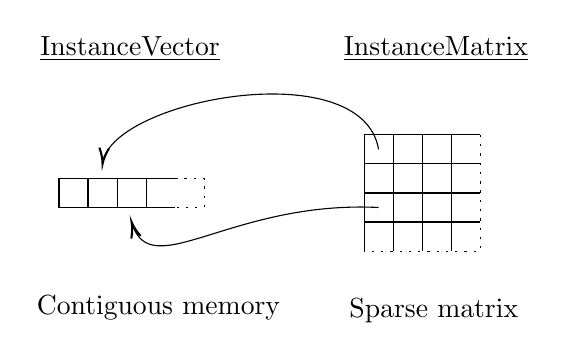
\begin{tikzpicture}[x=0.75pt,y=0.75pt,yscale=-.7,xscale=.7]
%uncomment if require: \path (0,300); %set diagram left start at 0, and has height of 300

%Straight Lines [id:da5639574855202493] 
\draw    (120,110) -- (100,110) -- (100,130) -- (120,130) ;


%Straight Lines [id:da3198582570446178] 
\draw    (140,110) -- (120,110) -- (120,130) -- (140,130) ;


%Straight Lines [id:da17404272158147815] 
\draw    (160,110) -- (140,110) -- (140,130) -- (160,130) ;


%Straight Lines [id:da13764436876683017] 
\draw    (180,110) -- (160,110) -- (160,130) -- (180,130) ;


%Straight Lines [id:da435813557354224] 
\draw  [dash pattern={on 0.84pt off 2.51pt}]  (180,110) -- (200,110) -- (200,130) -- (180,130) ;


%Shape: Grid [id:dp24563848864581883] 
\draw  [draw opacity=0] (310,80) -- (390,80) -- (390,160) -- (310,160) -- cycle ; \draw   (310,80) -- (310,160)(330,80) -- (330,160)(350,80) -- (350,160)(370,80) -- (370,160) ; \draw   (310,80) -- (390,80)(310,100) -- (390,100)(310,120) -- (390,120)(310,140) -- (390,140) ; \draw    ;
%Curve Lines [id:da8565130212882951] 
\draw    (320,90) .. controls (308.62,23.67) and (137.96,55.35) .. (130.19,98.68) ;
\draw [shift={(130,100)}, rotate = 275.84000000000003] [color={rgb, 255:red, 0; green, 0; blue, 0 }  ][line width=0.75]    (10.93,-3.29) .. controls (6.95,-1.4) and (3.31,-0.3) .. (0,0) .. controls (3.31,0.3) and (6.95,1.4) .. (10.93,3.29)   ;

%Curve Lines [id:da20453592495384287] 
\draw    (320,130) .. controls (218.52,125.05) and (163.6,182.83) .. (150.39,141.29) ;
\draw [shift={(150,140)}, rotate = 434.14] [color={rgb, 255:red, 0; green, 0; blue, 0 }  ][line width=0.75]    (10.93,-3.29) .. controls (6.95,-1.4) and (3.31,-0.3) .. (0,0) .. controls (3.31,0.3) and (6.95,1.4) .. (10.93,3.29)   ;

%Straight Lines [id:da09119048672720242] 
\draw  [dash pattern={on 0.84pt off 2.51pt}]  (390,80) -- (390,160) -- (310,160) ;


% Text Node
\draw (149,21) node  [align=left] {\underline{InstanceVector}};
% Text Node
\draw (359.5,21) node  [align=left] {\underline{InstanceMatrix}};
% Text Node
\draw (168.5,199) node  [align=left] {Contiguous memory};
% Text Node
\draw (358,201) node  [align=left] {Sparse matrix};

\end{tikzpicture}
\end{frame}

%%%%%%%%%%%%

\begin{frame}{Datastructures (2)}

Although there is some redundant storage, we combine the best of both storage types:\medskip
\begin{description}
\item[InstanceVector] Constant-time access by memory index, fast traversing in lexicographic order \bold{if sorted}.
\item[InstanceMatrix] Constant-time access by coordinate.
\end{description}\medskip
Need to manually manage the memory of the InstanceVector: adding/deleting/sorting changes indices and thus InstanceMatrix needs to be (completely) rebuild as well. Hence the need for \bold{refactoring}

\end{frame}

%%%%%%%%%%%%%

\begin{frame}{A practical algorithm (2)}

\tikzset{every picture/.style={line width=0.75pt}} %set default line width to 0.75pt        

\tiny
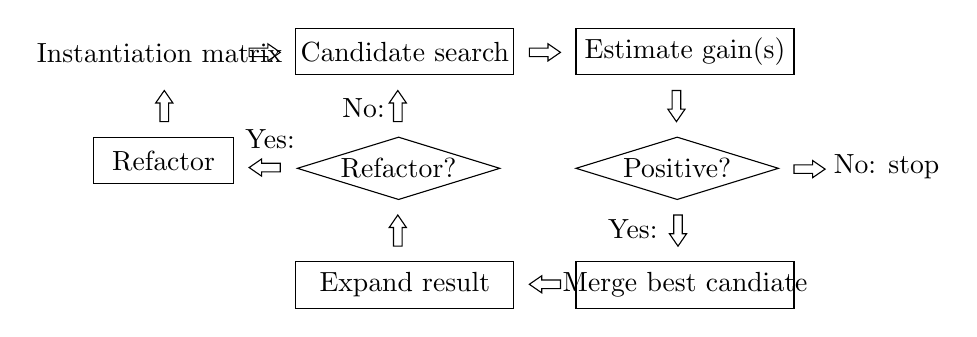
\begin{tikzpicture}[x=0.75pt,y=0.75pt,yscale=-.75,xscale=.75]
%uncomment if require: \path (0,300); %set diagram left start at 0, and has height of 300

%Flowchart: Process [id:dp4782497477496759] 
\draw   (200,60) -- (340,60) -- (340,90) -- (200,90) -- cycle ;
%Right Arrow [id:dp0106127781483073] 
\draw   (350,72.75) -- (362,72.75) -- (362,70) -- (370,75.5) -- (362,81) -- (362,78.25) -- (350,78.25) -- cycle ;
%Flowchart: Process [id:dp8391634624078887] 
\draw   (380,60) -- (520,60) -- (520,90) -- (380,90) -- cycle ;
%Right Arrow [id:dp2784645145213487] 
\draw   (447.25,100) -- (447.25,112) -- (450,112) -- (444.5,120) -- (439,112) -- (441.75,112) -- (441.75,100) -- cycle ;
%Flowchart: Process [id:dp41447896123303685] 
\draw   (380,210) -- (520,210) -- (520,240) -- (380,240) -- cycle ;
%Flowchart: Decision [id:dp26196178425216665] 
\draw   (445,130) -- (510,150) -- (445,170) -- (380,150) -- cycle ;
%Right Arrow [id:dp7826103447038623] 
\draw   (448.25,180) -- (448.25,192) -- (451,192) -- (445.5,200) -- (440,192) -- (442.75,192) -- (442.75,180) -- cycle ;
%Right Arrow [id:dp5430390369649105] 
\draw   (520,147.75) -- (532,147.75) -- (532,145) -- (540,150.5) -- (532,156) -- (532,153.25) -- (520,153.25) -- cycle ;
%Right Arrow [id:dp8544598770423162] 
\draw   (190,152.25) -- (178,152.25) -- (178,155) -- (170,149.5) -- (178,144) -- (178,146.75) -- (190,146.75) -- cycle ;
%Flowchart: Process [id:dp3531450147225088] 
\draw   (200,210) -- (340,210) -- (340,240) -- (200,240) -- cycle ;
%Right Arrow [id:dp5376430472123639] 
\draw   (262.75,200) -- (262.75,188) -- (260,188) -- (265.5,180) -- (271,188) -- (268.25,188) -- (268.25,200) -- cycle ;
%Flowchart: Decision [id:dp14752806042244282] 
\draw   (266,130) -- (331,150) -- (266,170) -- (201,150) -- cycle ;
%Right Arrow [id:dp8138585643184836] 
\draw   (262.75,120) -- (262.75,108) -- (260,108) -- (265.5,100) -- (271,108) -- (268.25,108) -- (268.25,120) -- cycle ;
%Right Arrow [id:dp9102501544724863] 
\draw   (170,72.75) -- (182,72.75) -- (182,70) -- (190,75.5) -- (182,81) -- (182,78.25) -- (170,78.25) -- cycle ;
%Flowchart: Process [id:dp10502859111005758] 
\draw   (70,130) -- (160,130) -- (160,160) -- (70,160) -- cycle ;
%Right Arrow [id:dp08006979212746357] 
\draw   (112.75,120) -- (112.75,108) -- (110,108) -- (115.5,100) -- (121,108) -- (118.25,108) -- (118.25,120) -- cycle ;
%Right Arrow [id:dp67324525964606] 
\draw   (370,227.25) -- (358,227.25) -- (358,230) -- (350,224.5) -- (358,219) -- (358,221.75) -- (370,221.75) -- cycle ;

% Text Node
\draw (270,75) node  [align=left] {Candidate search};
\draw (450,75) node  [align=left] {Estimate gain(s)};
\draw (450,225) node  [align=left] {Merge best candiate};
\draw (445,150) node  [align=left] {Positive?};
\draw (579.5,149) node  [align=left] {No: stop};
\draw (416.5,189) node  [align=left] {Yes:};
\draw (270,225) node  [align=left] {Expand result};
\draw (266,150) node  [align=left] {Refactor?};
\draw (243.5,111) node  [align=left] {No:};
\draw (112.5,76) node  [align=left] {Instantiation matrix};
\draw (115,145) node  [align=left] {Refactor};
\draw (183.5,131) node  [align=left] {Yes:};
\end{tikzpicture}
\end{frame}

%%%%%%%%%%%%%

\begin{frame}{A practical algorithm (2)}

\tikzset{every picture/.style={line width=0.75pt}} %set default line width to 0.75pt        

\tiny
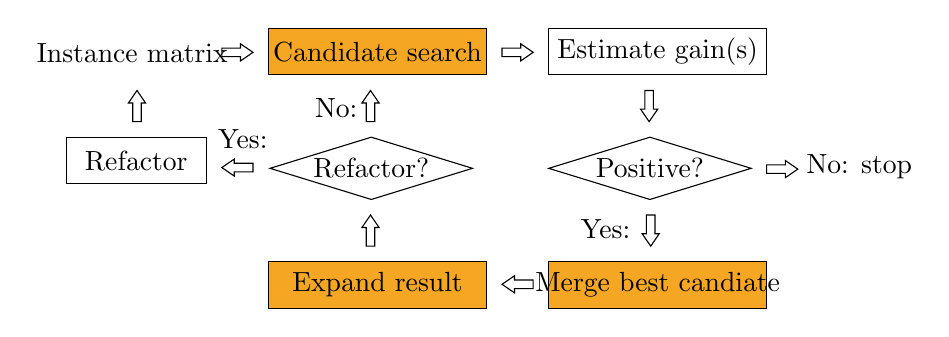
\begin{tikzpicture}[x=0.75pt,y=0.75pt,yscale=-.75,xscale=.75]
%uncomment if require: \path (0,300); %set diagram left start at 0, and has height of 300

%Flowchart: Process [id:dp4782497477496759] 
\draw  [fill={rgb, 255:red, 245; green, 166; blue, 35 }  ,fill opacity=1 ] (200,60) -- (340,60) -- (340,90) -- (200,90) -- cycle ;
%Right Arrow [id:dp0106127781483073] 
\draw   (350,72.75) -- (362,72.75) -- (362,70) -- (370,75.5) -- (362,81) -- (362,78.25) -- (350,78.25) -- cycle ;
%Flowchart: Process [id:dp8391634624078887] 
\draw   (380,60) -- (520,60) -- (520,90) -- (380,90) -- cycle ;
%Right Arrow [id:dp2784645145213487] 
\draw   (447.25,100) -- (447.25,112) -- (450,112) -- (444.5,120) -- (439,112) -- (441.75,112) -- (441.75,100) -- cycle ;
%Flowchart: Process [id:dp41447896123303685] 
\draw  [fill={rgb, 255:red, 245; green, 166; blue, 35 }  ,fill opacity=1 ] (380,210) -- (520,210) -- (520,240) -- (380,240) -- cycle ;
%Flowchart: Decision [id:dp26196178425216665] 
\draw   (445,130) -- (510,150) -- (445,170) -- (380,150) -- cycle ;
%Right Arrow [id:dp7826103447038623] 
\draw   (448.25,180) -- (448.25,192) -- (451,192) -- (445.5,200) -- (440,192) -- (442.75,192) -- (442.75,180) -- cycle ;
%Right Arrow [id:dp5430390369649105] 
\draw   (520,147.75) -- (532,147.75) -- (532,145) -- (540,150.5) -- (532,156) -- (532,153.25) -- (520,153.25) -- cycle ;
%Right Arrow [id:dp8544598770423162] 
\draw   (190,152.25) -- (178,152.25) -- (178,155) -- (170,149.5) -- (178,144) -- (178,146.75) -- (190,146.75) -- cycle ;
%Flowchart: Process [id:dp3531450147225088] 
\draw  [fill={rgb, 255:red, 245; green, 166; blue, 35 }  ,fill opacity=1 ] (200,210) -- (340,210) -- (340,240) -- (200,240) -- cycle ;
%Right Arrow [id:dp5376430472123639] 
\draw   (262.75,200) -- (262.75,188) -- (260,188) -- (265.5,180) -- (271,188) -- (268.25,188) -- (268.25,200) -- cycle ;
%Flowchart: Decision [id:dp14752806042244282] 
\draw   (266,130) -- (331,150) -- (266,170) -- (201,150) -- cycle ;
%Right Arrow [id:dp8138585643184836] 
\draw   (262.75,120) -- (262.75,108) -- (260,108) -- (265.5,100) -- (271,108) -- (268.25,108) -- (268.25,120) -- cycle ;
%Right Arrow [id:dp9102501544724863] 
\draw   (170,72.75) -- (182,72.75) -- (182,70) -- (190,75.5) -- (182,81) -- (182,78.25) -- (170,78.25) -- cycle ;
%Flowchart: Process [id:dp10502859111005758] 
\draw   (70,130) -- (160,130) -- (160,160) -- (70,160) -- cycle ;
%Right Arrow [id:dp08006979212746357] 
\draw   (112.75,120) -- (112.75,108) -- (110,108) -- (115.5,100) -- (121,108) -- (118.25,108) -- (118.25,120) -- cycle ;
%Right Arrow [id:dp67324525964606] 
\draw   (370,227.25) -- (358,227.25) -- (358,230) -- (350,224.5) -- (358,219) -- (358,221.75) -- (370,221.75) -- cycle ;

% Text Node
\draw (270,75) node  [align=left] {Candidate search};
% Text Node
\draw (450,75) node  [align=left] {Estimate gain(s)};
% Text Node
\draw (450,225) node  [align=left] {Merge best candiate};
% Text Node
\draw (445,150) node  [align=left] {Positive?};
% Text Node
\draw (579.5,149) node  [align=left] {No: stop};
% Text Node
\draw (416.5,189) node  [align=left] {Yes:};
% Text Node
\draw (270,225) node  [align=left] {Expand result};
% Text Node
\draw (266,150) node  [align=left] {Refactor?};
% Text Node
\draw (243.5,111) node  [align=left] {No:};
% Text Node
\draw (112.5,76) node  [align=left] {Instance matrix};
% Text Node
\draw (115,145) node  [align=left] {Refactor};
% Text Node
\draw (183.5,131) node  [align=left] {Yes:};


\end{tikzpicture}



\end{frame}

%%%%%%%%%%%%%

\begin{frame}{Candidate search}

A candidate can be defined as a tuple $<X,Y,\delta>$: two patterns and a relative offset between them. We derive a list of candidates from the instantiation matrix and count their \bold{usage}.

\newcommand{\ce}{\cellcolor{red!45!yellow}}
$$
\underbrace{
\begin{bmatrix}
\ce X & Y & X & Y & \ce X & X  \\[-.2em]
\ce X & \ce Y & X & X & Y & \ce Y  \\[-.2em]
Y & \ce Y & \ce X & X & X & Y  \\[-.2em]
X & X & X & \ce Y & X & X  \\[-.2em]
\ce X & X & X & X & \ce X & X  \\[-.2em]
X & \ce Y & X & X & X & \ce Y  \\
\end{bmatrix}}_{\textsf{Instantiation matrix}}
\longrightarrow
\underbrace{
\begin{matrix}
\cellcolor{red!45!yellow} X &   \\[-.2em]
 & \cellcolor{red!45!yellow}Y  \\[-.2em]
\end{matrix}}_{\textsf{Candidate}}
$$
\bigskip
Limitation: we only pick instances whose \emph{peripheries} overlap...

\end{frame}

%%%%%%%%%%%%%

\begin{frame}{Peripheries}

Along with its elements, we store each pattern's \bold{periphery}:

\newcommand{\Ant}{\cellcolor{red!45!yellow}\cdot}
\newcommand{\Post}{\cellcolor{teal!75}\cdot}

$$
\begin{matrix}
\ddots & \vdots & \vdots & \vdots & \vdots & \vdots & \iddots \\[-.2em]
\cdots & \cdot & \cdot & \cdot & \cdot & \cdot & \cdots \\[-.2em]
\cdots & \cdot & \Ant  & \Ant  & \Ant  & \Ant  & \cdots \\[-.2em]
\cdots & \cdot & \Ant  & x_{0,0}& x_{0,1}& \Post & \cdots \\[-.2em]
\cdots & \cdot & \Ant  & x_{1,0}& x_{1,1}& \Post & \cdots \\[-.2em]
\cdots & \cdot & \Post & \Post & \Post & \Post & \cdots \\[-.2em]
\cdots & \cdot & \cdot & \cdot & \cdot & \cdot & \cdots \\[-.4em]
\iddots & \vdots & \vdots & \vdots & \vdots & \vdots & \ddots
\end{matrix}
$$

The periphery elements are used to look in the neighbourhood of an instance.

\end{frame}


%%%%%%%%%%%%%

\begin{frame}{Peripheries (2)}

During candidate search, we are only looking in the \bold{posterior periphery}. Consider the first iteration (only singletons):

\newcommand{\Ant}{\cellcolor{red!45!yellow}\cdot}
\newcommand{\Post}{\cellcolor{teal!75}\cdot}

$$
\begin{matrix}
\ddots & \vdots & \vdots & \vdots & \vdots & \iddots \\[-.2em]
\cdots & \cdot & \cdot & \cdot & \cdot & \cdots \\[-.2em]
\cdots & \cdot & \cdot & \cdot & \cdot & \cdots \\[-.2em]
\cdots & \cdot & \cdot  & x    & \Post & \cdots \\[-.2em]
\cdots & \cdot & \Post & \Post & \Post & \cdots \\[-.2em]
\cdots & \cdot & \cdot & \cdot & \cdot & \cdots \\[-.4em]
\iddots & \vdots & \vdots & \vdots & \vdots & \ddots
\end{matrix}
$$

Given a total number of unique elements $n$, we can produce up to $4n^2$ candidates (phew!). So for example, our noise image could give us $4(256)^2=262144$ candidates in the first iteration alone...

\end{frame}

%%%%%%%%%%%%%

\begin{frame}{Overlap}

Counting candidates is not so simple, however.\\ How many times do you see $\begin{matrix}
1 &   \\[-.2em]
 & 1  \\[-.2em]
\end{matrix}$

$$
\begin{matrix}
\ddots & \vdots & \vdots & \vdots & \vdots & \vdots & \iddots \\[-.2em]
\cdots & 1     & \cdot & \cdot & \cdot & \cdot  & \cdots \\[-.2em]
\cdots & \cdot & 1     & \cdot & \cdot & \cdot & \cdots \\[-.2em]
\cdots & \cdot & \cdot & 1    & \cdot & \cdot & \cdots \\[-.2em]
\cdots & \cdot & \cdot & \cdot & 1    & \cdot & \cdots \\[-.2em]
\cdots & \cdot & \cdot & \cdot & \cdot & 1   &  \cdots \\[-.4em]
\iddots & \vdots & \vdots & \vdots & \vdots & \vdots & \ddots
\end{matrix}
$$

Four can be counted, but at most two pairs can be merged. Solution: storing per-instance \bold{overlap coefficients}.

\end{frame}


%%%%%%%%%%%%%


\begin{frame}{Overlap (2)}

\newcommand{\Ant}{\cellcolor{red!45!yellow}\cdot}
\newcommand{\Post}{\cellcolor{teal!75}\cdot}

Computing the overlap coefficient $c$.\bigskip

\tikzset{every picture/.style={line width=0.75pt}} %set default line width to 0.75pt        

\small\centering
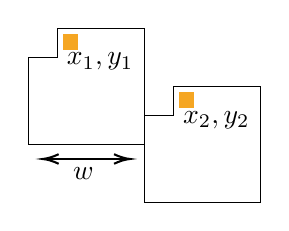
\begin{tikzpicture}[x=0.75pt,y=0.75pt,yscale=-.7,xscale=.7]
%uncomment if require: \path (0,300); %set diagram left start at 0, and has height of 300

%Shape: Polygon [id:ds2691035906427982] 
\draw   (60,70) -- (60,50) -- (120,50) -- (120,130) -- (40,130) -- (40,70) -- cycle ;
%Shape: Rectangle [id:dp3235546855370074] 
\draw  [draw opacity=0][fill={rgb, 255:red, 245; green, 166; blue, 35 }  ,fill opacity=1 ] (64,54) -- (74,54) -- (74,65) -- (64,65) -- cycle ;
%Shape: Polygon [id:ds07051932220581003] 
\draw   (140,110) -- (140,90) -- (200,90) -- (200,170) -- (120,170) -- (120,110) -- cycle ;
%Shape: Rectangle [id:dp4816752667989629] 
\draw  [draw opacity=0][fill={rgb, 255:red, 245; green, 166; blue, 35 }  ,fill opacity=1 ] (144,94) -- (154,94) -- (154,105) -- (144,105) -- cycle ;
%Straight Lines [id:da11862334463628654] 
\draw    (52,140) -- (108,140) ;
\draw [shift={(110,140)}, rotate = 180] [color={rgb, 255:red, 0; green, 0; blue, 0 }  ][line width=0.75]    (10.93,-3.29) .. controls (6.95,-1.4) and (3.31,-0.3) .. (0,0) .. controls (3.31,0.3) and (6.95,1.4) .. (10.93,3.29)   ;
\draw [shift={(50,140)}, rotate = 0] [color={rgb, 255:red, 0; green, 0; blue, 0 }  ][line width=0.75]    (10.93,-3.29) .. controls (6.95,-1.4) and (3.31,-0.3) .. (0,0) .. controls (3.31,0.3) and (6.95,1.4) .. (10.93,3.29)   ;

% Text Node
\draw (89.5,73) node  [align=left] {$\displaystyle x_{1} ,y_{1}$};
% Text Node
\draw (169.5,113) node  [align=left] {$\displaystyle x_{2} ,y_{2}$};
% Text Node
\draw (78,150) node  [align=left] {$\displaystyle w$};


\end{tikzpicture}


$$
c = w + x_2 - x_1 + (y_2 - y_1)(2w + 1)
$$


\end{frame}

%%%%%%%%%%%%%

\begin{frame}{Overlap (3)}

To each instance $\bar{X}$ we add an \bold{overlap bitvector} $V()$. The candidate search algorithm now looks like this. \medskip 

We visit every instance $\bar{X}\in\bar{H}$ in lexicographical order. Then for each $\bar{X}$ we look at all instances $\bar{Y}$ that we can reach from the posterior periphery of $X$:

\begin{description}
\item[1] if $X\neq Y$, goto 6.
\item[2] With the offset between $\bar{X}$ and $\bar{Y}$ we obtain candidate $<X,Y,\delta>$:
\item[3] Compute the overlap coefficient $c$ from $\delta$
\item[4] If $\bar{X}$ has $V(c)$ set to 1, skip this candidate
\item[5] Otherwise set $V(c)$ on $\bar{Y}$ to 1 
\item[6] Increment the usage of $<X,Y,\delta>$ by one
\end{description}

\end{frame}

%%%%%%%%%%%%%

\begin{frame}{A practical algorithm (3)}

\tikzset{every picture/.style={line width=0.75pt}} %set default line width to 0.75pt        

\tiny
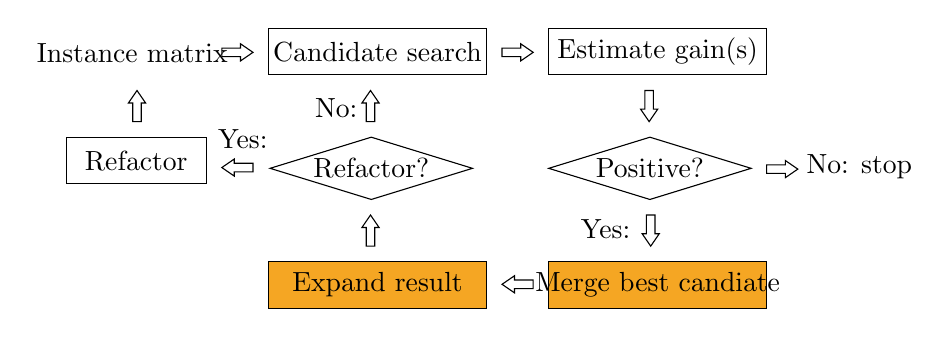
\begin{tikzpicture}[x=0.75pt,y=0.75pt,yscale=-.75,xscale=.75]
%uncomment if require: \path (0,300); %set diagram left start at 0, and has height of 300

%Flowchart: Process [id:dp4782497477496759] 
\draw   (200,60) -- (340,60) -- (340,90) -- (200,90) -- cycle ;
%Right Arrow [id:dp0106127781483073] 
\draw   (350,72.75) -- (362,72.75) -- (362,70) -- (370,75.5) -- (362,81) -- (362,78.25) -- (350,78.25) -- cycle ;
%Flowchart: Process [id:dp8391634624078887] 
\draw   (380,60) -- (520,60) -- (520,90) -- (380,90) -- cycle ;
%Right Arrow [id:dp2784645145213487] 
\draw   (447.25,100) -- (447.25,112) -- (450,112) -- (444.5,120) -- (439,112) -- (441.75,112) -- (441.75,100) -- cycle ;
%Flowchart: Process [id:dp41447896123303685] 
\draw  [fill={rgb, 255:red, 245; green, 166; blue, 35 }  ,fill opacity=1 ] (380,210) -- (520,210) -- (520,240) -- (380,240) -- cycle ;
%Flowchart: Decision [id:dp26196178425216665] 
\draw   (445,130) -- (510,150) -- (445,170) -- (380,150) -- cycle ;
%Right Arrow [id:dp7826103447038623] 
\draw   (448.25,180) -- (448.25,192) -- (451,192) -- (445.5,200) -- (440,192) -- (442.75,192) -- (442.75,180) -- cycle ;
%Right Arrow [id:dp5430390369649105] 
\draw   (520,147.75) -- (532,147.75) -- (532,145) -- (540,150.5) -- (532,156) -- (532,153.25) -- (520,153.25) -- cycle ;
%Right Arrow [id:dp8544598770423162] 
\draw   (190,152.25) -- (178,152.25) -- (178,155) -- (170,149.5) -- (178,144) -- (178,146.75) -- (190,146.75) -- cycle ;
%Flowchart: Process [id:dp3531450147225088] 
\draw  [fill={rgb, 255:red, 245; green, 166; blue, 35 }  ,fill opacity=1 ] (200,210) -- (340,210) -- (340,240) -- (200,240) -- cycle ;
%Right Arrow [id:dp5376430472123639] 
\draw   (262.75,200) -- (262.75,188) -- (260,188) -- (265.5,180) -- (271,188) -- (268.25,188) -- (268.25,200) -- cycle ;
%Flowchart: Decision [id:dp14752806042244282] 
\draw   (266,130) -- (331,150) -- (266,170) -- (201,150) -- cycle ;
%Right Arrow [id:dp8138585643184836] 
\draw   (262.75,120) -- (262.75,108) -- (260,108) -- (265.5,100) -- (271,108) -- (268.25,108) -- (268.25,120) -- cycle ;
%Right Arrow [id:dp9102501544724863] 
\draw   (170,72.75) -- (182,72.75) -- (182,70) -- (190,75.5) -- (182,81) -- (182,78.25) -- (170,78.25) -- cycle ;
%Flowchart: Process [id:dp10502859111005758] 
\draw   (70,130) -- (160,130) -- (160,160) -- (70,160) -- cycle ;
%Right Arrow [id:dp08006979212746357] 
\draw   (112.75,120) -- (112.75,108) -- (110,108) -- (115.5,100) -- (121,108) -- (118.25,108) -- (118.25,120) -- cycle ;
%Right Arrow [id:dp67324525964606] 
\draw   (370,227.25) -- (358,227.25) -- (358,230) -- (350,224.5) -- (358,219) -- (358,221.75) -- (370,221.75) -- cycle ;

% Text Node
\draw (270,75) node  [align=left] {Candidate search};
% Text Node
\draw (450,75) node  [align=left] {Estimate gain(s)};
% Text Node
\draw (450,225) node  [align=left] {Merge best candiate};
% Text Node
\draw (445,150) node  [align=left] {Positive?};
% Text Node
\draw (579.5,149) node  [align=left] {No: stop};
% Text Node
\draw (416.5,189) node  [align=left] {Yes:};
% Text Node
\draw (270,225) node  [align=left] {Expand result};
% Text Node
\draw (266,150) node  [align=left] {Refactor?};
% Text Node
\draw (243.5,111) node  [align=left] {No:};
% Text Node
\draw (112.5,76) node  [align=left] {Instance matrix};
% Text Node
\draw (115,145) node  [align=left] {Refactor};
% Text Node
\draw (183.5,131) node  [align=left] {Yes:};


\end{tikzpicture}

\end{frame}

%%%%%%%%%%%%%

\begin{frame}{Merging candidates}

Assume that the pattern we are trying to find contains $N$ elements, it takes ...
\begin{itemize}
\item At most $N-1$ merges,
\item At least $\log_2(N)$ merges ...
\end{itemize}
... to construct it from singletons.\medskip

Unfortunately, in practice we get $N-1$ rather than $\log_2(N)$.
\end{frame}

%%%%%%%%%%%%%

\begin{frame}{Flood-fill}

We can try to approach $\log_2(N)$ by implementing a local search.\
Say we merge candidate $<X,Y,\delta>$ into pattern $Z$, now for all resulting instances $\bar{Z}_i \in \bar{Z}_0,\bar{Z}_1,\dots\bar{Z}_{m-1}$:
$$
W = \ominus(\bar{H}_{\delta_0 + c}) \iff \forall \bar{Z}_i \cdot \ominus(\bar{H}_{\delta_i + c}) = W
$$
Where $\delta_i$ is the offset of $\bar{Z}_i$ and $c$ is an element from the periphery of $Z$. If such $W$ exists, replace all instances $\bar{Z}$ with the respective unions $\bar{Z}+\bar{W}$.
\end{frame}

%%%%%%%%%%%%%

\begin{frame}{Flood-fill (2)}

So when merging $X$ and $Y$ below, we look at the \emph{resulting} periphery to see what adjacent pattern(s) \emph{all instances} have in common.

\newcommand{\Ant}{\cellcolor{red!45!yellow}\cdot}
\newcommand{\Post}{\cellcolor{teal!75}\cdot}

$$
\begin{matrix}
\ddots & \vdots & \vdots & \vdots & \vdots & \vdots & \iddots \\[-.2em]
\cdots & \cdot & \cdot & \cdot & \cdot & \cdot & \cdots \\[-.2em]
\cdots & \cdot & \Ant  & \Ant  & \cdot & \cdot  & \cdots \\[-.2em]
\cdots & \cdot & \Ant  & X     & \Post & \Post & \cdots \\[-.2em]
\cdots & \cdot & \Ant  & \Ant  & Y      & \Post & \cdots \\[-.2em]
\cdots & \cdot & \cdot & \Post & \Post & \Post & \cdots \\[-.2em]
\cdots & \cdot & \cdot & \cdot & \cdot & \cdot & \cdots \\[-.4em]
\iddots & \vdots & \vdots & \vdots & \vdots & \vdots & \ddots
\end{matrix}
$$

We simply add all resulting matches, recursively. This result in a BFS, or 'flood fill'.

\end{frame}

%%%%%%%%%%%%%

\begin{frame}{Merging candidates (2)}

Candidate search is expensive, so we try to merge more candidates per iteration.\medskip

We keep a set of used patterns $P_{used}$ and initialize it to $\emptyset$. Now for each candidate $<X,Y,\delta>$ in the list of candidates:
\begin{itemize}
\item If either $X\in P_{used}$ or $Y \in P_{used}$, skip
\item Otherwise, merge the candidate
\item Add $X$ and $Y$ to $P_{used}$
\end{itemize}

This is indeed a different heuristic that leads to slightly different results.

\end{frame}

%%%%%%%%%%%%%

\begin{frame}{Pre-processing}

VOUW utilized two simple data pre-processing steps.
\begin{itemize}
\item Quantization: limit the number of singletons to begin with
\item `Tabu' patterns: exclude very prevalent singletons 
\end{itemize}

Both steps have a profound effect on the results and there is no `one size fits all'.

\end{frame}

%%%%%%%%%%%%%

\begin{frame}{Tabu patterns}

\newcommand{\ca}{\cellcolor{cyan!45!yellow}}
\newcommand{\cb}{\cellcolor{red!75!blue}}
\newcommand{\cc}{\cellcolor{violet}}
\newcommand{\cd}{\cellcolor{teal!75}}
\newcommand{\ce}{\cellcolor{red!45!yellow}}

\small
$$
\begin{matrix}
\ce 1 & \ce 1 & \cd 0 & \cd 0 & \ce 1  \\
\ce 1 & \cd 0 & \ce 1 & \ce 1 & \cd 0  \\
\cd 0 & \cd 0 & \ce 1 & \cd 0 & \ce 1  \\
\ce 1 & \ce 1 & \ce 1 & \ce 1 & \cd 0  \\
\ce 1 & \cd 0 & \ce 1 & \cd 0 & \cd 0  \\
\end{matrix}
\ \rightarrow \
\begin{matrix}
\ca 1 & \ca 1 & \cd 0 & \cd 0 & \ce 1  \\
\ce 1 & \cd 0 & \ca 1 & \ca 1 & \cd 0  \\
\cd 0 & \cd 0 & \ce 1 & \cd 0 & \ce 1  \\
\ca 1 & \ca 1 & \ca 1 & \ca 1 & \cd 0  \\
\ce 1 & \cd 0 & \ce 1 & \cd 0 & \cd 0  \\
\end{matrix}
\ \rightarrow \
\begin{matrix}
\ca 1 & \ca 1 & \cd 0 & \cd 0 & \ce 1  \\
\cb 1 & \cb 0 & \ca 1 & \ca 1 & \cd 0  \\
\cd 0 & \cd 0 & \cb 1 & \cb 0 & \ce 1  \\
\ca 1 & \ca 1 & \ca 1 & \ca 1 & \cd 0  \\
\cb 1 & \cb 0 & \cb 1 & \cb 0 & \cd 0  \\
\end{matrix}
\ \rightarrow \
\begin{matrix}
\cc 1 & \cc 1 & \cd 0 & \cd 0 & \ce 1  \\
\cc 1 & \cc 0 & \cc 1 & \cc 1 & \cd 0  \\
\cd 0 & \cd 0 & \cc 1 & \cc 0 & \ce 1  \\
\cc 1 & \cc 1 & \cc 1 & \cc 1 & \cd 0  \\
\cc 1 & \cc 0 & \cc 1 & \cc 0 & \cd 0  \\
\end{matrix}
$$

With `0' removed from the matrix

\small
$$
\begin{matrix}
\ce 1 & \ce 1 & \cdot & \cdot & \ce 1  \\
\ce 1 & \cdot & \ce 1 & \ce 1 & \cdot  \\
\cdot & \cdot & \ce 1 & \cdot & \ce 1  \\
\ce 1 & \ce 1 & \ce 1 & \ce 1 & \cdot  \\
\ce 1 & \cdot & \ce 1 & \cdot & \cdot  \\
\end{matrix}
\ \rightarrow \
\begin{matrix}
\ca 1 & \ca 1 & \cdot & \cdot & \ce 1  \\
\ce 1 & \cdot & \ca 1 & \ca 1 & \cdot  \\
\cdot & \cdot & \ce 1 & \cdot & \ce 1  \\
\ca 1 & \ca 1 & \ca 1 & \ca 1 & \cdot  \\
\ce 1 & \cdot & \ce 1 & \cdot & \cdot  \\
\end{matrix}
\ \rightarrow \
\begin{matrix}
\cc 1 & \cc 1 & \cdot & \cdot & \ce 1  \\
\cc 1 & \cdot & \cc 1 & \cc 1 & \cdot  \\
\cdot & \cdot & \cc 1 & \cdot & \ce 1  \\
\cc 1 & \cc 1 & \cc 1 & \cc 1 & \cdot  \\
\cc 1 & \cdot & \cc 1 & \cdot & \cdot  \\
\end{matrix}
$$

\end{frame}

%%%%%%%%%%%%%

\begin{frame}{Problem classes}

Not all matrices and patterns are equally difficult for VOUW. They can roughly be divided in five classes.
\begin{description}
\item[Class 1a] Exact duplicates in a sparse matrix.
\item[Class 1b] Exact duplicates in (differently distributed) noise.
\item[Class 1c] Exact duplicates in noise with equal distribution.
\item[Class 2 ] Approximate duplicates
\item[Class 3 ] Transformed duplicates
\end{description}

\end{frame}

%%%%%%%%%%%%%

\begin{frame}{Future goals}

\begin{center}
\includegraphics[width=0.4\paperwidth]{"VOUW logo-02"} 
\end{center}

\begin{itemize}
\item Implement at least the ability to solve the `class 2' problem.
\item Rethink the encoding scheme, it is still not good enough ;-)
\item Finish writing the paper.
\end{itemize}\bigskip

\emph{Thank you for your attention!}

\end{frame}

%%%%%%%%%%%%%

\end{document}